\clearpage
\cleardoublepage

\chapter{神经网络核心操作}

\section{引言}

本章涵盖现代神经网络的基本构建模块：卷积、池化和归一化操作。理解这些操作对于设计和实现有效的神经网络架构至关重要。

\section{卷积操作}

卷积是卷积神经网络（CNN）的基石。

\subsection{2D卷积}

对于输入 $\mathbf{X} \in \mathbb{R}^{H \times W}$ 和卷积核 $\mathbf{K} \in \mathbb{R}^{K \times K}$：
\begin{equation}
y[i,j] = \sum_{m=0}^{K-1}\sum_{n=0}^{K-1} k[m,n] \cdot x[i+m, j+n]
\end{equation}

在实践中，我们通常添加偏置并使用多个卷积核产生多个输出通道。

\begin{properties}[卷积参数]
\begin{itemize}
    \item \textbf{卷积核大小：}$K \times K$（常见：$3\times3$、$5\times5$、$7\times7$）
    \item \textbf{步长（$s$）：}滑动窗口的步长
    \item \textbf{填充（$p$）：}输入周围的零填充
    \item \textbf{膨胀（$d$）：}卷积核元素之间的间距
\end{itemize}
\end{properties}

带填充和步长的输出尺寸：
\begin{equation}
H_{out} = \left\lfloor \frac{H_{in} + 2p - d(K-1) - 1}{s} + 1 \right\rfloor
\end{equation}

\begin{figure}[htbp]
    \centering
    \begin{tikzpicture}[scale=0.7]
        % 带填充的输入
        \foreach \x in {0,...,4} {
            \foreach \y in {0,...,4} {
                \ifthenelse{\x < 1 \OR \x > 3 \OR \y < 1 \OR \y > 3}
                {\fill[gray!30] (\x, \y) +(-0.4, -0.4) rectangle ++(0.4, 0.4);}
                {\fill[blue!50] (\x, \y) +(-0.4, -0.4) rectangle ++(0.4, 0.4);}
            }
        }
        \node at (2, -1) {输入 $5\times5$ 带填充};
        
        % 卷积核
        \foreach \x in {0,...,2} {
            \foreach \y in {0,...,2} {
                \fill[red!50] (7+\x, 2+\y) +(-0.4, -0.4) rectangle ++(0.4, 0.4);
            }
        }
        \node at (8, 0.5) {$3\times3$ 卷积核};
        
        % 输出
        \foreach \x in {0,...,2} {
            \foreach \y in {0,...,2} {
                \fill[green!50] (7+\x, -3+\y) +(-0.4, -0.4) rectangle ++(0.4, 0.4);
            }
        }
        \node at (8, -5) {$3\times3$ 输出};
        
        % 步长1
        \node[draw, dashed, red] at (1.5, 2.5) {};
        \node[draw, dashed, red] at (2.5, 2.5) {};
        \node[draw, dashed, red] at (3.5, 2.5) {};
    \end{tikzpicture}
    \caption{带填充的卷积}
    \label{fig:conv_padding}
\end{figure}

\subsection{分组卷积和深度卷积}

\begin{itemize}
    \item \textbf{分组卷积：}将输入通道分成组，分别对每组应用卷积
    \item \textbf{深度卷积：}每个输入通道一个卷积核（分组数 $G = C_{in}$）
    \item \textbf{逐点卷积：}$1\times1$ 卷积（用于混合通道）
\end{itemize}

MobileNet使用：深度可分离卷积 = 深度卷积 + 逐点卷积

\begin{properties}[深度可分离卷积]
\begin{itemize}
    \item \textbf{标准卷积FLOPs：}$H \cdot W \cdot K^2 \cdot C_{in} \cdot C_{out}$
    \item \textbf{可分离卷积FLOPs：}$H \cdot W \cdot K^2 \cdot C_{in} + H \cdot W \cdot C_{in} \cdot C_{out}$
    \item \textbf{加速比：}大约 $\frac{1}{K^2} + \frac{1}{C_{out}}$
\end{itemize}
\end{properties}

\subsection{空洞（带孔）卷积}

空洞卷积在卷积核元素之间插入零，在不增加参数数量或计算量的情况下扩展感受野：

\begin{equation}
y[i,j] = \sum_{m=0}^{K-1}\sum_{n=0}^{K-1} k[m,n] \cdot x[i + m \cdot d, j + n \cdot d]
\end{equation}
其中 $d$ 是膨胀率。

\begin{properties}[空洞卷积特性]
\begin{itemize}
    \item \textbf{带膨胀 $d$ 的感受野：}有效卷积核大小 $= d(K - 1) + 1$
    \item \textbf{FLOPs：}与标准卷积相同（只有采样模式改变）
    \item \textbf{参数：}与标准卷积相同
    \item \textbf{关键应用：}语义分割（DeepLab系列），需要大感受野而不使用池化或步长
\end{itemize}
\end{properties}

\begin{example}[堆叠空洞卷积]
三个膨胀率 $d = 1, 2, 4$ 的 $3 \times 3$ 卷积产生总感受野：
\begin{equation}
\text{RF} = 1 + (3-1)\times1 + (3-1)\times2 + (3-1)\times4 = 15
\end{equation}
这与单个 $15 \times 15$ 标准卷积的感受野匹配，但只有 $3 \times 9C^2$ 参数而非 $225C^2$。这是\textbf{DeepLab} \cite{chen2017deeplab} 的核心思想。
\end{example}

\section{池化操作}

池化减少空间维度并提供平移不变性。

\subsection{最大池化}

\begin{equation}
y[i,j] = \max_{m,n \in \mathcal{N}(i,j)} x[m,n]
\end{equation}

其中 $\mathcal{N}(i,j)$ 是邻域。

\begin{itemize}
    \item \textbf{保留最强激活}
    \item \textbf{提供局部平移不变性}
    \item \textbf{常见：}$2\times2$ 步长2
\end{itemize}

\subsection{平均池化}

\begin{equation}
y[i,j] = \frac{1}{K \cdot K}\sum_{m,n \in \mathcal{N}(i,j)} x[m,n]
\end{equation}

\begin{itemize}
    \item \textbf{对邻域平均}
    \item \textbf{比最大池化保守}
    \item \textbf{用于全局池化}
\end{itemize}

\begin{figure}[htbp]
    \centering
    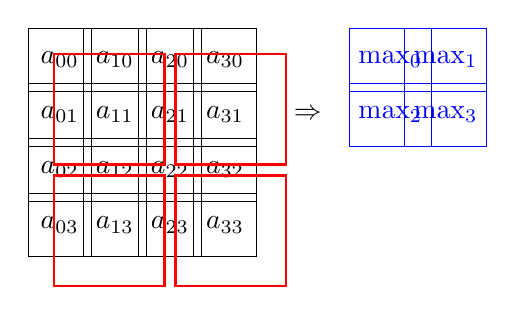
\begin{tikzpicture}[scale=0.7]
        % 输入
        \foreach \x in {0,...,3} {
            \foreach \y in {0,...,3} {
                \node[draw, minimum size=0.8cm] at (\x, -\y) {$a_{\x\y}$};
            }
        }
        
        % 最大池化框
        \draw[red, thick] (-0.1, 0.1) rectangle (1.9, -1.9);
        \draw[red, thick] (2.1, 0.1) rectangle (4.1, -1.9);
        \draw[red, thick] (-0.1, -2.1) rectangle (1.9, -4.1);
        \draw[red, thick] (2.1, -2.1) rectangle (4.1, -4.1);
        
        \node at (4.5, -1) {$\Rightarrow$};
        
        % 输出
        \node[draw, blue, minimum size=0.8cm] at (6, 0) {$\max_0$};
        \node[draw, blue, minimum size=0.8cm] at (7, 0) {$\max_1$};
        \node[draw, blue, minimum size=0.8cm] at (6, -1) {$\max_2$};
        \node[draw, blue, minimum size=0.8cm] at (7, -1) {$\max_3$};
    \end{tikzpicture}
    \caption[最大池化 2x2, 步长2]{最大池化 $2\times2$，步长2}
    \label{fig:maxpool}
\end{figure}

\subsection{全局池化}

应用于整个特征图以产生每个通道的单个值：
\begin{itemize}
    \item \textbf{全局平均池化（GAP）：}$\frac{1}{HW}\sum_{i,j} x_{ij}$
    \item \textbf{全局最大池化：}$\max_{i,j} x_{ij}$
    \item \textbf{替代 FC 层}在现代架构中
\end{itemize}

\section{归一化技术}

归一化通过控制层输入分布来稳定训练。

\subsection{批归一化}

在批次维度上归一化激活：
\begin{equation}
\hat{x}_i = \frac{x_i - \mu_B}{\sqrt{\sigma_B^2 + \epsilon}}, \quad y_i = \gamma \hat{x}_i + \beta
\end{equation}

其中：
\begin{align}
\mu_B &= \frac{1}{m}\sum_{i=1}^{m} x_i \\
\sigma_B^2 &= \frac{1}{m}\sum_{i=1}^{m}(x_i - \mu_B)^2
\end{align}

\begin{properties}[BatchNorm特性]
\begin{itemize}
    \item \textbf{减少内部协变量偏移}
    \item \textbf{允许更高的学习率}
    \item \textbf{提供轻微的正则化}
    \item \textbf{依赖批次大小，小批次可能有问题}
\end{itemize}
\end{properties}

\begin{note}[BatchNorm vs 推理]
训练期间，BatchNorm 使用批次统计。推理期间，使用运行统计：
\begin{equation}
\hat{x} = \frac{x - \tilde{\mu}}{\sqrt{\tilde{\sigma}^2 + \epsilon}}
\end{equation}
其中 $\tilde{\mu}$ 和 $\tilde{\sigma}^2$ 是运行均值。
\end{note}

\subsection{层归一化}

对单个样本内的特征进行归一化：
\begin{equation}
\mu = \frac{1}{D}\sum_{i=1}^{D} x_i, \quad \sigma = \frac{1}{D}\sum_{i=1}^{D}(x_i - \mu)^2
\end{equation}

\begin{itemize}
    \item \textbf{独立于批次大小}
    \item \textbf{用于 RNN 和 Transformer}
    \item \textbf{训练和推理时相同}
\end{itemize}

\begin{table}[ht]
    \centering
    \caption{归一化比较}
    \begin{tabular}{L{2cm} L{2.5cm} L{2.5cm} L{3cm}}
        \toprule
        \textbf{方法} & \textbf{归一化维度} & \textbf{依赖批次} & \textbf{用例} \\
        \midrule
        BatchNorm & $(H, W, C)$ & 是 & CNN \\
        LayerNorm & $(H, W, N)$ & 否 & Transformer \\
        InstanceNorm & $(H, W)$ & 否 & 风格迁移 \\
        GroupNorm & $(H, W, G)$ & 否 & 小批次CNN \\
        \bottomrule
    \end{tabular}
\end{table}

\subsection{实例归一化}

独立归一化每个样本和通道：
\begin{equation}
y_{nchw} = \frac{x_{nchw} - \mu_{nc}}{\sqrt{\sigma_{nc}^2 + \epsilon}}
\end{equation}

用于风格迁移，其中实例特定的统计信息很重要。

\subsection{组归一化}

组归一化（GN）将通道分成 $G$ 组，分别独立地对每组进行归一化 \cite{wu2018group}。这提供了一个统一框架，将 LayerNorm 和 InstanceNorm 作为特例。

对于形状为 $(N, C, H, W)$ 的张量，每组 $C/G$ 个通道：
\begin{align}
\mu_g &= \frac{1}{(C/G) \cdot H \cdot W} \sum_{c \in \mathcal{G}_g} \sum_{h,w} x_{nchw} \\
\sigma_g^2 &= \frac{1}{(C/G) \cdot H \cdot W} \sum_{c \in \mathcal{G}_g} \sum_{h,w} (x_{nchw} - \mu_g)^2 \\
\hat{x}_{nchw} &= \frac{x_{nchw} - \mu_g}{\sqrt{\sigma_g^2 + \epsilon}}
\end{align}

\begin{properties}[GN作为统一框架]
\begin{itemize}
    \item $G = 1$：GroupNorm 变为\textbf{LayerNorm}（跨所有通道归一化）
    \item $G = C$：GroupNorm 变为\textbf{InstanceNorm}（逐通道归一化）
    \item $G = 32$ 是大多数实现中的默认值（一个好的权衡）
    \item \textbf{独立于批次大小：}与批次大小1一起工作（例如医学成像）
    \item 计算量与 BatchNorm 等价；只有分组改变
\end{itemize}
\end{properties}

\begin{table}[ht]
    \centering
    \caption{归一化方法：统一视图}
    \begin{tabular}{L{2cm} L{3cm} L{2cm} L{3.5cm}}
        \toprule
        \textbf{方法} & \textbf{统计量计算维度} & \textbf{依赖批次} & \textbf{主要用途} \\
        \midrule
        BatchNorm & $(N, H, W)$ 每 $C$ & 是 & CNN（大批次） \\
        LayerNorm & $(H, W, C)$ 每 $N$ & 否 & Transformer, RNN \\
        InstanceNorm & $(H, W)$ 每 $N,C$ & 否 & 风格迁移 \\
        GroupNorm & $(H, W, C/G)$ 每 $N$ & 否 & 检测、小批次 \\
        \bottomrule
    \end{tabular}
\end{table}

\section{正则化操作}

除了归一化之外，几种操作通过在训练期间引入随机性或约束来防止过拟合。

\subsection{Dropout}

Dropout \cite{srivastava2014dropout} 在训练期间以概率 $p$ 随机将激活置零：
\begin{equation}
\tilde{x}_i = \frac{m_i \cdot x_i}{1 - p}, \quad m_i \sim \text{Bernoulli}(1 - p)
\end{equation}
缩放因子 $1/(1-p)$（倒置 dropout）确保 $\mathbb{E}[\tilde{x}_i] = x_i$，因此推理时不需要调整。

\subsubsection{为什么Dropout有效：贝叶斯解释}

Dropout 可以被视为近似贝叶斯推断 \cite{gal2016dropout}。每个 dropout 掩码定义一个不同的子网络，训练带 dropout 等同于：
\begin{equation}
p(\mathbf{y} \mid \mathbf{x}, \mathcal{D}) \approx \frac{1}{T}\sum_{t=1}^{T} p(\mathbf{y} \mid \mathbf{x}, \mathbf{W} \odot \mathbf{m}^{(t)})
\end{equation}
这是在指数数量的稀疏网络（$N$ 个单元为 $2^N$）上进行\textbf{模型平均}，通过方差减少提高泛化。

\subsubsection{Dropout变体}

\begin{table}[ht]
    \centering
    \caption{Dropout变体}
    \begin{tabular}{L{3cm} L{4.5cm} L{4.5cm}}
        \toprule
        \textbf{变体} & \textbf{操作} & \textbf{用例} \\
        \midrule
        标准Dropout & 以概率 $p$ 将激活置零 & FC层 \\
        DropConnect & 以概率 $p$ 将\textbf{权重}置零 & FC层 \\
        Spatial Dropout & 将整个特征图置零 & CNN \\
        DropPath & 跳过整个路径/块 & 深度网络 \\
        DropBlock & 丢弃连续区域 & CNN（正则化） \\
        \bottomrule
    \end{tabular}
\end{table}

\textbf{DropPath}（随机深度）\cite{huang2016deep} 在训练期间随机跳过整个残差块。对于输入 $\mathbf{x}$ 和输出 $\mathcal{F}(\mathbf{x})$ 的块：
\begin{equation}
\tilde{\mathbf{y}} = \begin{cases} \mathbf{x} & \text{以概率 } p_L \\ \mathcal{F}(\mathbf{x}) + \mathbf{x} & \text{以概率 } 1 - p_L \end{cases}
\end{equation}
丢弃率 $p_L$ 通常随深度线性增加，创建在训练期间作为集成起作用的更短有效网络。

\section{组合操作}

现代网络将这些操作组合成标准化的块。

\subsection{基本卷积块}

典型的卷积块：
\begin{enumerate}
    \item 卷积
    \item 批归一化
    \item 激活（ReLU/GELU）
\end{enumerate}

常见模式：
\begin{itemize}
    \item Conv-BN-ReLU（VGG风格）
    \item BN-ReLU-Conv（ResNet风格，预激活）
\end{itemize}

\begin{code}
    \captionof{listing}{PyTorch中的卷积块}
    \label{code:conv_block}
\begin{lstlisting}[language=python]
import torch.nn as nn

class ConvBlock(nn.Module):
    def __init__(self, in_ch, out_ch, kernel_size=3, stride=1):
        super().__init__()
        padding = kernel_size // 2
        self.block = nn.Sequential(
            nn.Conv2d(in_ch, out_ch, kernel_size, stride, padding, bias=False),
            nn.BatchNorm2d(out_ch),
            nn.ReLU(inplace=True)
        )
    
    def forward(self, x):
        return self.block(x)

# 预激活块（ResNet风格）
class PreActBlock(nn.Module):
    def __init__(self, in_ch, out_ch, stride=1):
        super().__init__()
        self.block = nn.Sequential(
            nn.BatchNorm2d(in_ch),
            nn.ReLU(inplace=True),
            nn.Conv2d(in_ch, out_ch, 3, stride, 1, bias=False),
            nn.BatchNorm2d(out_ch),
            nn.ReLU(inplace=True),
            nn.Conv2d(out_ch, out_ch, 3, 1, 1, bias=False)
        )
        self.shortcut = nn.Identity() if stride==1 and in_ch==out_ch else \
                        nn.Conv2d(in_ch, out_ch, 1, stride, bias=False)
    
    def forward(self, x):
        return self.block(x) + self.shortcut(x)
\end{lstlisting}
\end{code}

\section{本章小结}

\begin{enumerate}
    \item 卷积用共享权重提取局部特征
    \item 深度可分离卷积为移动部署减少计算
    \item 空洞卷积在不增加额外参数的情况下扩展感受野
    \item 池化提供空间缩减和不变性
    \item 归一化稳定训练动态（CNN用BN，Transformer用LN，小批次用GN）
    \item Dropout及其变体通过随机深度提供正则化
    \item 现代架构将这些组合成标准化的块
    \item 操作的选择取决于任务和数据特性
\end{enumerate}

\section{扩展阅读}

\begin{itemize}
    \item \cite{srivastava2014dropout} --- Dropout：防止神经网络过拟合的简单方法
    \item \cite{ioffe2015batch} --- 批归一化：通过减少内部协变量偏移加速深度网络训练
    \item \cite{ba2016layer} --- 层归一化
    \item \cite{gal2016dropout} --- Dropout作为贝叶斯近似
    \item \cite{huang2016deep} --- 带随机深度的深度网络
    \item \cite{chen2017deeplab} --- 重新思考用于语义图像分割的空洞卷积
    \item \cite{howard2017mobilenets} --- MobileNets：用于移动视觉应用的高效CNN
    \item \cite{wu2018group} --- 组归一化
\end{itemize}

\section{习题}

\begin{enumerate}
    \item \textbf{卷积输出尺寸：}对于输入尺寸 $32\times32$、卷积核大小5、填充2、步长1和膨胀1，计算输出高度和宽度。对步长2重复计算。

    \item \textbf{深度可分离FLOPs：}对于输入形状 $56\times56\times64$ 和输出通道128，比较标准 $3\times3$ 卷积与深度可分离卷积的FLOPs。

    \item \textbf{空洞感受野：}三个 $3\times3$ 卷积使用膨胀率 $1, 2, 4$。推导有效感受野并解释为什么这在语义分割中有用。

    \item \textbf{池化选择：}比较包含一个强激活和许多弱激活的特征图上的最大池化和平均池化。哪种操作更好地保留显著的局部证据？

    \item \textbf{归一化策略：}你的GPU内存只允许检测模型的批次大小为2。你会选择 BatchNorm、LayerNorm 还是 GroupNorm？解释权衡。

    \item \textbf{Dropout实践：}为什么通常在推理时禁用 dropout？推导为什么倒置dropout在训练期间保持预期激活不变。
\end{enumerate}
